%
% $Id$
% 
%       This source code is part of
% 
%        G   R   O   M   A   C   S
% 
% GROningen MAchine for Chemical Simulations
% 
%               VERSION 2.0
% 
% Copyright (c) 1991-1999
% BIOSON Research Institute, Dept. of Biophysical Chemistry
% University of Groningen, The Netherlands
% 
% Please refer to:
% GROMACS: A message-passing parallel molecular dynamics implementation
% H.J.C. Berendsen, D. van der Spoel and R. van Drunen
% Comp. Phys. Comm. 91, 43-56 (1995)
% 
% Also check out our WWW page:
% http://md.chem.rug.nl/~gmx
% or e-mail to:
% gromacs@chem.rug.nl
% 
% And Hey:
% Giving Russians Opium May Alter Current Situation
%

\section{Parallel Molecular Dynamics}
In this chapter we describe some details of the \swapindex{parallel}{MD}  
algorithm used 
in {\gromacs}. This also includes some other information on neighbor searching and
a side excursion to parallel sorting.
Please note the following which we use throughout this chapter:\\
{\bf definition:} {\natom}: Number of particles, {\nproc} number of processors.\\
{\gromacs} employs two different grids: the neighbor searching grid ({\nsgrid})
and the combined charge/po\-ten\-tial grid ({\fftgrid}), as will be described below.
To maximize the confusion, 
these two grids are mapped onto a grid of processors when {\gromacs} runs on a 
parallel computer.

\subsection{Domain decomposition}
Modern day parallel computers, such as an IBM SP/2 or a Cray T3E
consist of relatively small numbers of relatively fast scalar
processors (typically 8 to 256).  The communication channels that are
available in hardware on these machine are not directly visible for
the programmer, a software layer (usually \normindex{MPI}) 
hides this, and makes communication from all processors to all
others possible. In contrast, in the {\gromacs} hardware~\cite{Berendsen95a}
only communication in a ring was available, {\ie} each processor could communicate
with its direct neighbors only.

It seems logical to map the computational box of an MD simulation system 
to a 3D grid of 
processors ({\eg} 4x4x4 for a 64 processor system). This ensures that most 
interactions that are local in space can be computed with information from 
neighboring processors only. However, this means that there have to be
communication channels in 3 dimensions too, which is not necessarily the case.
Although this may be overcome in software, such a mapping is complicated for the MD
software as well, without clear benefits in terms of performance for most
parallel computers. 

Therefore we opt for a simple one-dimensional division scheme
for the computational box. Each processor gets a slab of this box in the 
X-dimension.
For the communication between processors this has two main advantages:
\begin{enumerate}
\item   Simplicity of coding. Communication can only be to two neighbors
        (called {\em left} and {\em right} in {\gromacs}).
\item   Communication can usually be done in large chunks, which makes it
        more efficient on most hardware platforms.
\end{enumerate}

Most interactions in molecular dynamics have in principle a short ranged character.
Bonds, angles and dihedrals are guaranteed to have the corresponding particles 
close in space.


\subsection{Domain decomposition for non-bonded forces}
For large parallel computers, domain decomposition is preferable over particle
decomposition, since it is easier to do load balancing. Without load balancing
the scaling of the code is rather poor...
For this purpose, the computational box is divided in {\nproc} slabs, where {\nproc}
is equal to the number of processors. There are multiple ways of dividing the box
over processors, but since the {\gromacs} code assumes
a ring topology for the processors, it is logical to cut the system in slabs in
just one dimension, the X dimension. 
The algorithm for neighbor searching then becomes:
\begin{enumerate}
\item   Make a list of charge group indices sorted on (increasing) X coordinate
        (\figref{parsort}).
        {\bf Note} that care must be taken to parallelize the sorting algorithm
        as well. See \secref{parsort}.
\item   Divide this list into slabs, such that each slab has the same number of
        charge groups
\item   Put the particles corresponding to the local slab on a 3D {\nsgrid} as 
        described in \secref{nsgrid}.
\item   Communicate the {\nsgrid} to neighboring processors (not necessarily to all
        processors). The amount of neighboring {\nsgrid} cells (N$_{gx}$) to 
        communicate is determined by the cut-off length $r_c$ according to
        \beq
        N_{gx}  ~=~     \frac{r_c \nproc}{l_x}   
        \eeq
        where $l_x$ is the box length in the slabbing direction. 
\item   On each processor compute the neighbor list for all charge groups in
        its slab using the normal grid neighbor-searching.
\end{enumerate}

\begin{figure}
\centerline{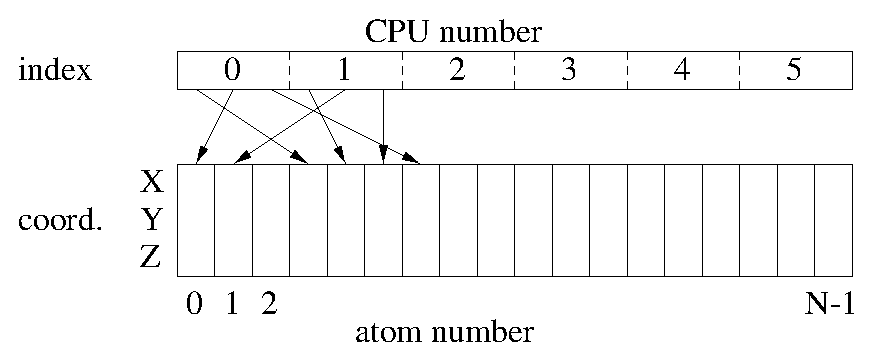
\includegraphics[width=10cm]{plots/parsort}}
\caption[Index in the coordinate array.]{Index in the coordinate
array. The division in slabs is indicated by dashed lines.}
\label{fig:parsort}
\end{figure}

For homogeneous system, this is close to an optimal load balancing,
without actually doing load balancing. For inhomogeneous system, such
as membranes, or interfaces, the dimension for slabbing must be chosen
such that it is perpendicular to the interface; in this fashion each
processor has ``a little bit of everything''.  The {\gromacs} utility
program {\tt editconf} has an option to rotate a whole
computational box.

The following observations are important here:
\begin{itemize}
\item   Particles may diffuse from one slab to the other, therefore each processor
        must hold coordinates for all particles all the time, and distribute forces
        back to all processors as well.
\item   Velocities are kept on the ``home processor'' for each particle,
        where the integration of Newton's equations is done.
\item   Fixed interaction lists (bonds, angles etc.) are kept each
        on a single processor.  Since all processors have all
        coordinates, it does not matter where interactions are
        calculated.  The division is actually done by the {\gromacs}
        preprocessor {\tt grompp} and care is taken that, as far as
        possible, every processor gets the same number of bonded
        interactions.
\end{itemize}

In all, this makes for a mixed particle decomposition/domain decomposition scheme
for parallelization of the MD code. The communication costs are four times higher
than for the simple particle decomposition method described in \secref{par}
(the whole coordinate and force array are communicated across the whole ring,
rather than half the array over half the ring).
However, for large numbers of processors the improved load balancing 
compensates this easily.

\subsection{Parallel \normindex{PPPM}}
A further reason for domain decomposition is the PPPM algorithm. This
algorithm works with a 3D Fast Fourier Transform. It employs a
discrete grid of dimensions (\nx,\ny,\nz), the {\fftgrid}. The
algorithm consist of five steps, each of which have to be
parallelized:
\begin{enumerate}
\item   Spreading charges on the {\fftgrid} to obtain the charge 
        distribution $\rho(\ve{r})$.
        This bit involves the following sub-steps:
        \begin{enumerate}
        \item[{\bf a.}] put particle in the box
        \item[{\bf b.}] find the {\fftgrid} cell in which the particle resides
        \item[{\bf c.}] add the charge of the particle times the appropriate
                        weight factor (see \secref{pppm}) to 
                        each of the 27 grid points (3 x 3 x 3).
        \end{enumerate}
        In the parallel case, the {\fftgrid} 
        must be filled on each processor with its
        share of the particles, and subsequently the {\fftgrid}s of all processors
        must be summed to find the total charge distribution. It may be clear that
        this induces a large amount of unnecessary work, unless we use domain
        decomposition. If each processor only has particles in a certain region
        of space, it only has to calculate the charge distribution for 
        that region of space. Since {\gromacs} works with slabs, this means that
        each processor fills the {\fftgrid} cells corresponding to it's slab in space
        and addition of {\fftgrid}s need only be done for neighboring slabs.\\
        To be more precise, the slab $x$ for processor $i$ is defined as:
        \beq
        i\, \frac{l_x}{M} \le x <\, (i+1)\frac{l_x}{M}
        \eeq
        Particle with this $x$ coordinate range will add to the charge distribution
        on the following range of 
        of {\fftgrid} slabs in the $x$ direction:
        \beq
        {\rm trunc}\left(i\,\frac{l_x \nx}{M}\right)-1 \le i_x \le {\rm trunc}\left((i+1)\,\frac{l_x \nx}{M}\right)+2
        \eeq
        where trunc indicates the truncation of a real number to the largest integer
        smaller than or equal to that real number.
        
\item   Doing the Fourier transform of the charge distribution $\rho(\ve{r})$ 
        in parallel to obtain $\hat{\rho}(\ve{k})$. This is done using
        the FFTW library (see \href{http://www.fftw.org}{www.fftw.org})
        which employs the MPI library for message passing programs
        (note that there are also \swapindex{shared}{memory} versions
        of the FFTW code).\\
        This FFT algorithm actually use slabs as well (good
        thinking!).  Each processor does 2D FFTS on its slab, and then
        the whole {\fftgrid} is transposed {\em in place}
        ({\ie} without using extra memory).  This means that after the
        FFT the X and Y components are swapped.  To complete the FFT,
        this swapping should be undone in principle (by transposing
        back).  Happily the FFTW code has an option to omit this,
        which we use in the next step.
\item   Convolute $\hat{\rho}(\ve{k})$ with the Fourier transform of the
        charge spread function $\hat{g}(\ve{k})$ (which we have tabulated before)
        to obtain the potential $\hat{\phi}(k)$. 
        As an optimization, we store the $\hat{g}(\ve{k})$  in transposed form
        as well, matching the transposed form of $\hat{\rho}(\ve{k})$
        which we get from the FFTW routine. After this step we have the 
        potential $\hat{\phi}(k)$ in Fourier space, but still on the transposed
        {\fftgrid}.
\item   Do an inverse transform of $\hat{\phi}(k)$ to obtain
        ${\phi}(\ve{r})$. Since the algorithm must do a transpose of the data
        this step actually yields the wanted result: the un-transposed
        potential in real space.
\item   Interpolate the potential ${\phi}(\ve{r})$ in real space at the particle
        positions to obtain forces and energy. For this bit the same considerations
        towards parallelism hold as for the charge spreading. However in this
        case more neighboring grid cells are needed, such that we need
        the following set of {\fftgrid} slabs in the $x$ direction:
        \beq
        {\rm trunc}\left(i\,\frac{l_x \nx}{M}\right)-3 \le i_x \le {\rm trunc}\left((i+1)\,\frac{l_x \nx}{M}\right)+4
        \eeq

\end{enumerate}
The algorithm as sketched above requires communication for spreading
the charges, for the FFTW forward and backward, and for interpolating
the forces.  The {\gromacs} bits of the program use only left and
right communication, {\ie}  using two communication channels. The FFTW
routines actually use other forms of communication as well, and these
routines are coded with MPI routines for message passing. This implies
that {\gromacs} can only perform the PPPM algorithm on parallel
computers computers that support MPI. However, most
\swapindex{shared}{memory} computers, such as the SGI Origin also
support MPI using the 
shared memory for communication.

\subsection{Parallel sorting}
\label{sec:parsort}
For the domain decomposition bit of {\gromacs} it is necessary to sort the 
coordinates (or rather the index to coordinates) every time a neighbor list is made.
If we use brute force, and sort all coordinates on each processor (which is 
technically possible since we have all the coordinates), then this sorting procedure
will take a constant time (proportional to {\natom}$^2\log${\natom}, 
independent of the number of processors. We can however do a little
better, if we assume that particles diffuse only slowly.
A parallel sorting algorithm can be conceived as follows: \\
At the first step of the simulation
\begin{enumerate}
\item   Do a full sort of all indices using {\eg} the  quick-sort algorithm that is
        built-in in the standard C-library
\item   Divide the sorted array into slabs (as described above see 
        \figref{parsort}).
\end{enumerate}
At subsequent steps of the simulation:
\begin{enumerate}
\item   Send the indices for each processor to the preceding processor (if
        not processor 0) and to the next processor (if not {\nproc}-1). The 
        communication associated with this operation is proportional to
        2{\natom}/{\nproc}.
\item   Sort the combined indices of the three (or two) processors. Note that
        the CPU time associated with sorting is now
        (3{\natom}/{\nproc})$^2\log$ (3{\natom}/{\nproc}).
\item   On each processor, the indices belonging to it's slab can be determined
        from the order of the array (\figref{parsort}).
\end{enumerate}

%\section{A Worked Example}
%Suppose our box size is 4.0 nm and the cut-off is 0.8 nm. For neighborsearching 
%we use {\dgrid} = 2, such that there 10 {\nsgrid} cells.
